\section{概率校准与分类决策}
\label{sec:classification-calibration}

前面各节在“两类误判代价相同、按最大得分或概率判类”的约定下比较模型。实际决策中，把负类误判为正类（误报）与把正类漏判为负类（漏报）的后果通常不同：拦截正常邮件、放走垃圾邮件、拒绝合规申请、误报安全风险，代价量级并不对称。这时“预测类别”只是决策的一步，还需要先有可靠的置信度量，再按代价选择动作。本节集中讲三件公共的事：概率输出怎样与误判代价对接、温度缩放怎样事后调整置信度、从训练到校准再到测试怎样完整验证。它们与具体二分类器无关，OvR、Softmax、SVM得分或朴素贝叶斯后验都可能用到同一套决策流程。

\subsection{概率输出与误判代价}
\label{sec:classification-cost-decision}

\subsubsection{从模型输出到可用信息}
记正类后验概率为$p(\bm x)=\mathbb P(Y=1\mid\bm X=\bm x)$。给定一个待决策动作，期望代价是把每个动作在各类下的代价按后验加权。设预测正类时误报代价为$a>0$（真实为负类却判正类），预测负类时漏报代价为$r>0$（真实为正类却判负类），正确分类代价为零。在$\bm x$处：
\[
\begin{aligned}
\text{判正类的期望代价}
  &=a\,(1-p(\bm x)),\\
\text{判负类的期望代价}
  &=r\,p(\bm x).
\end{aligned}
\]

\subsubsection{给定类别概率的代价最小化}
选择期望代价较小的动作，即判正类当且仅当$a(1-p)\leq rp$，整理得
\begin{equation}
  p(\bm x)\geq \tau=\frac{a}{a+r}.
  \label{eq:classification-cost-threshold}
\end{equation}
两类代价相等（$a=r$）时$\tau=1/2$，回到最大概率判类；误报代价越高，判正类所需的概率门槛越高。例如教学设定$a=4$、$r=1$，则$\tau=4/5=0.8$，必须有八成以上把握才预测正类。

在对数几率尺度上，等价的得分阈值更直观。若$p=\sigma(z)$，则$p\geq\tau$等价于$z\geq\log[\tau/(1-\tau)]$。$a=4,r=1$时$\tau=0.8$，对应得分阈值$\log(0.8/0.2)=\log4\approx1.386$：线性得分至少达到这个值才触发正类动作。

图\ref{fig:classification-logistic-probability}把概率阈值与得分阈值放在同一条S形曲线上比较：曲线本身没有改变，改变的只是把概率转成动作的门槛。

\begin{figure}[htbp]
  \centering
  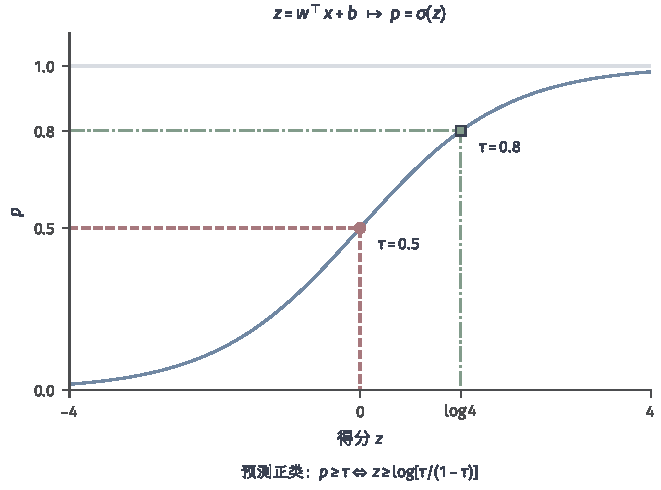
\includegraphics[width=105.412mm]{figures/07-classic-models/00-shared/matplotlib/classification-logistic-probability/figure.pdf}
  \caption{线性得分$z=\bm{w}^{\top}\bm{x}+b$经Logistic函数转为正类概率$p$。蓝色实线为$p=\sigma(z)$；红色虚线与圆点标出$(0,0.5)$，绿色点划线与方点标出$(\log4,0.8)$。两组辅助线分别连接概率阈值与对应的得分阈值，数值是教学构造，不表示训练或校准结果。}
  \label{fig:classification-logistic-probability}
\end{figure}

式\eqref{eq:classification-cost-threshold}有一个前提：式中的$p(\bm x)$必须是可靠的类别后验。若模型只是把得分压缩到$(0,1)$而未经校准（下一节），真实频率与报告概率对不上，按代价算出的门槛就会偏。代价由决策问题给出，不能由训练数据估计；它可以直接改变阈值而不必重训模型，但若从建树或训练起就按加权误分类率学习，得到的是另一个学习目标，两者不是同一过程。

\subsection{概率校准与温度缩放}
\label{sec:classification-temperature}

\subsubsection{校准对象与数据分工}
Softmax输出满足概率公理（非负、和为一），却不自动满足\term{概率校准}（probability calibration）：在报告某类概率约为$0.8$的一组样本中，该类的实际比例也应接近$0.8$。有限样本、模型失配、正则化和分布变化都可能破坏这种对应。这里检验的是报告概率与实际频率的联系，和按最大概率选择类别是不同的问题。分类正确只要求最高概率胜出，概率质量则要求报告的置信度对得上真实频率，二者可能分开失败。

\subsubsection{冻结得分的温度缩放}
一种简洁的后处理是\term{温度缩放}（temperature scaling）：固定已训练得分$z_c(\bm x)$，只学习一个标量温度$T>0$，令
\begin{equation}
  \tilde p_c(\bm x)
  =\frac{\exp(z_c(\bm x)/T)}
         {\sum_{r=1}^{C}\exp(z_r(\bm x)/T)}.
  \label{eq:classification-temperature-softmax}
\end{equation}
$T=1$时回到原Softmax；$T>1$把得分除以更大的数，指数差被压缩，概率分布更平缓（更不确定）；$T<1$则使分布更尖锐。因为分子分母同除以$T$，最高得分类别不变，所以温度缩放不改变分类决策，只改变置信度的集中程度。

温度在一份未参与原模型拟合的校准记录上估计。令校准集为$\{(\bm x_i,y_i)\}_{i=1}^{m}$，对每个样本计算式\eqref{eq:classification-temperature-softmax}，最小化多类负对数似然（NLL）：
\begin{equation}
  L(T)=-\sum_{i=1}^{m}\log\tilde p_{y_i}(\bm x_i;T).
  \label{eq:classification-temperature-nll}
\end{equation}
求导得到单变量优化。记$z_{i,c}=z_c(\bm x_i)$，$p_{i,c}=\tilde p_c(\bm x_i;T)$，则
\begin{equation}
  \frac{\partial L}{\partial T}
  =\frac{1}{T^2}\sum_{i=1}^{m}
    \left[z_{i,y_i}-\sum_{c=1}^{C}p_{i,c}z_{i,c}\right].
  \label{eq:classification-temperature-derivative}
\end{equation}
括号内是真实类得分减去按当前温度加权的平均得分；令梯度为零即得到最优温度的隐式方程，可用一维搜索（如 Brent 法）求解，无须改动原模型参数。

\subsubsection{分别评价概率与类别决策}
概率质量还可用\term{Brier分数}（Brier score）直接度量：
\begin{equation}
  \operatorname{BS}
  =\frac{1}{m}\sum_{i=1}^{m}
    \sum_{c=1}^{C}
      [p_{i,c}-\mathbb 1\{y_i=c\}]^2,
  \label{eq:classification-brier}
\end{equation}
它衡量预测概率向量与独热标签向量的平方偏差，越小越好。NLL对错误的高置信预测惩罚更重，Brier分数对整体偏差更平滑，两者可同时报告。

Guo等在其研究的网络和数据上比较了温度缩放与其他校准方法；单一温度是全局标量，不能修复所有概率失配，类别间或区域间的系统性偏差需要更灵活的校准映射\scite{guo2017calibration}。

\subsection{完整分类流程的验证与使用}
\label{sec:classification-pipeline}

校准与代价决策必须在独立于拟合过程的数据上评价，否则会把训练集的乐观偏差误认为可靠。完整流程把数据切成三份：

\begin{enumerate}
  \item \textbf{训练集}：拟合模型参数（权重、分裂、原型等），得到原始得分$z_c(\bm x)$。
  \item \textbf{校准集}：固定训练好的模型，只在这份数据上估计温度$T$（或其他校准映射），并检查NLL、Brier分数与可靠性图。
  \item \textbf{测试集}：按既定代价$\tau$（式\eqref{eq:classification-cost-threshold}）输出动作，在完全未参与拟合与校准的数据上报告期望代价、各类错误与概率质量。
\end{enumerate}

三份数据的角色不能互换：用训练集估温会让温度迎合拟合误差，用测试集选温则使测试集不再是独立评价。数据量不足时，可用交叉验证在各折内分别完成“训练—校准—测试”，再汇总指标。代价$\tau$由业务给出，不参与任何拟合；报告时应同时给出分类错误、期望决策代价和校准指标，避免只看准确率就宣称概率可靠。
